% MICRO 2026 Survey Paper - ML Performance Models
% Using MICRO 59 ACM sigconf template
% Last compiled: 2026-02-07 (rebuild triggered)

%%
%% For submission and review of your manuscript please change the
%% command to \documentclass[manuscript, screen, review]{acmart}.
%%
\documentclass[sigconf, screen, review]{acmart}

%%
%% \BibTeX command to typeset BibTeX logo in the docs
\AtBeginDocument{%
  \providecommand\BibTeX{{%
    Bib\TeX}}}

%% Rights management information - for submission
\setcopyright{none}
\copyrightyear{2026}
\acmYear{2026}
\acmDOI{}

%% Conference information
\acmConference[MICRO 2026]{The 59th IEEE/ACM International Symposium on Microarchitecture}{November 2026}{Austin, TX, USA}
\acmISBN{}

%% Disable ACM reference format printing for submission
\settopmatter{printfolios=true}
\settopmatter{printacmref=false}

%% Anonymous submission
\author{Anonymous Author(s)}
\affiliation{%
  \institution{Under Review}
  \country{Anonymous}
}

%% Additional packages (acmart already loads amsmath, amsfonts, amssymb, booktabs)
\usepackage{multirow}
\usepackage{tikz}
\usetikzlibrary{shapes.geometric,arrows.meta,positioning,fit,backgrounds,patterns}
\usepackage{pgfplots}
\pgfplotsset{compat=1.18}
\usepgfplotslibrary{groupplots}
\usetikzlibrary{plotmarks}

% Custom commands
\newcommand{\todo}[1]{\textcolor{red}{[TODO: #1]}}

\begin{document}

\title{A Survey of High-Level Modeling and Simulation Methods for Modern Machine Learning Workloads}
\subtitle{\normalsize{MICRO 2026 Submission -- Confidential Draft -- Do NOT Distribute!!}}

%%
%% The abstract is a short summary of the work to be presented in the
%% article.

%%%%%% -- PAPER CONTENT STARTS-- %%%%%%%%

\begin{abstract}
As machine learning workloads grow in scale and complexity---spanning training and inference for CNNs, transformers, mixture-of-experts models, and LLMs---architects and system designers need fast, accurate methods to predict their performance across diverse hardware platforms.
This survey provides a comprehensive analysis of the tools and methods available for modeling and simulating the performance of ML workloads, covering analytical models, cycle-accurate simulators, trace-driven approaches, and ML-augmented hybrid techniques.
We survey over 30 tools drawn from 53 papers across architecture venues (MICRO, ISCA, HPCA, ASPLOS) and systems venues (MLSys, OSDI, NSDI) published between 2016--2026, spanning DNN accelerator modeling (Timeloop, MAESTRO, Sparseloop), GPU simulation (GPGPU-Sim, Accel-Sim, NeuSight), distributed training simulation (ASTRA-sim, Lumos, SimAI), and LLM inference serving (VIDUR, Frontier, AMALI).
We organize the literature along three dimensions---methodology type (analytical, simulation, ML-augmented, hybrid), target platform (accelerators, GPUs, distributed systems, edge devices), and abstraction level (kernel, model, system)---while additionally characterizing tools by workload coverage, revealing a pervasive CNN-validation bias.
Our analysis reveals that hybrid approaches combining analytical structure with learned components achieve the best accuracy-speed trade-offs, while pure analytical models offer superior interpretability for design space exploration.
We conduct hands-on reproducibility evaluations of five representative tools, finding that reproducibility varies dramatically: Docker-first tools score 8.5+/10 on our rubric while tools relying on serialized ML models risk becoming unusable.
We identify key open challenges including cross-workload generalization beyond CNNs, composition of kernel-level predictions to end-to-end accuracy, and support for emerging architectures.
This survey provides practitioners guidance for selecting appropriate modeling tools and researchers a roadmap for advancing the field of ML workload performance prediction.
\end{abstract}

%%
%% Keywords
\keywords{ML workload performance prediction, DNN accelerator modeling, GPU simulation, distributed training simulation, LLM inference serving, design space exploration, survey}

\maketitle

% ==============================================================================
% INTRODUCTION
% ==============================================================================
\section{Introduction}
\label{sec:introduction}

Machine learning workloads---spanning training and inference for CNNs, transformers, mixture-of-experts models, and graph neural networks---have become the dominant consumers of compute across datacenters and edge devices.
The shift toward domain-specific architectures~\cite{hennessy2019golden}, from Google's TPU~\cite{tpuv1_2017,tpuv4_2023} to custom training accelerators, has created a heterogeneous hardware landscape where architects and system designers need fast, accurate performance predictions to navigate vast design spaces, select parallelization strategies, provision serving infrastructure, and optimize hardware-software co-design.
Yet ML workloads pose unique modeling challenges: they exhibit diverse computational patterns (dense matrix operations in attention layers, sparse accesses in GNNs, communication-bound collective operations in distributed training) across this increasingly heterogeneous landscape of GPUs, TPUs, custom accelerators, and multi-device clusters.

A rich ecosystem of tools has emerged, spanning analytical models (Timeloop~\cite{timeloop2019}, MAESTRO~\cite{maestro2019}: 5--10\% error at microsecond speed), cycle-accurate simulators (GPGPU-Sim~\cite{gpgpusim2009}, Accel-Sim~\cite{accelsim2020}: detailed but hours per workload), trace-driven simulators (ASTRA-sim~\cite{astrasim2023}, VIDUR~\cite{vidur2024}: system-scale training and serving), and ML-augmented hybrid approaches (NeuSight~\cite{neusight2025}: 2.3\% error on GPU kernels).
Each methodology occupies a distinct point in the accuracy-speed-generality trade-off space.

Despite this rich tool landscape, no comprehensive survey organizes these methods from the perspective of the ML workload practitioner---the architect or engineer who needs to select a modeling tool for a specific design or deployment task.
Existing surveys focus on ML \emph{techniques} for performance modeling~\cite{granite2022} or on specific hardware targets~\cite{timeloop2019}, leaving practitioners without guidance on which tools suit their needs across the full modeling spectrum.
This survey fills that gap by providing a methodology-centric view of the tools and methods available for predicting ML workload performance.

We make the following contributions:
\begin{itemize}
    \item A \textbf{methodology-centric taxonomy} organizing tools along three dimensions: methodology type (analytical, simulation, ML-augmented, hybrid), target platform (DNN accelerators, GPUs, distributed systems, edge devices), and abstraction level (kernel, model, system), with a quantitative coverage matrix identifying research gaps and a workload coverage analysis exposing the CNN-validation bias in the literature.
    \item A \textbf{systematic survey} of over 30 modeling tools drawn from 53 papers across architecture venues (MICRO, ISCA, HPCA, ASPLOS) and systems venues (MLSys, OSDI, NSDI) published between 2016--2026, using documented selection criteria.
    \item A \textbf{comparative analysis} examining trade-offs between accuracy, speed, generalization, and interpretability, with careful qualification of paper-reported accuracy claims and identification of cases where reported numbers are unverifiable.
    \item \textbf{Hands-on reproducibility evaluations} of representative tools with a 10-point rubric, and identification of \textbf{open challenges} including the CNN-to-transformer generalization gap, kernel-to-end-to-end error composition, and emerging accelerator support.
\end{itemize}

The paper proceeds as follows: Section~\ref{sec:methodology} describes our methodology; Section~\ref{sec:background} provides background; Section~\ref{sec:taxonomy} presents the taxonomy; Section~\ref{sec:survey} surveys tools by platform; Section~\ref{sec:comparison} compares accuracy and provides tool selection guidance; Section~\ref{sec:evaluation} presents reproducibility evaluations; Section~\ref{sec:challenges} discusses open challenges; and Section~\ref{sec:conclusion} concludes.

Figure~\ref{fig:timeline} illustrates the evolution of performance modeling tools for ML workloads, from early analytical frameworks through simulators to modern hybrid approaches.

\begin{figure}[t]
\centering
\resizebox{\columnwidth}{!}{%
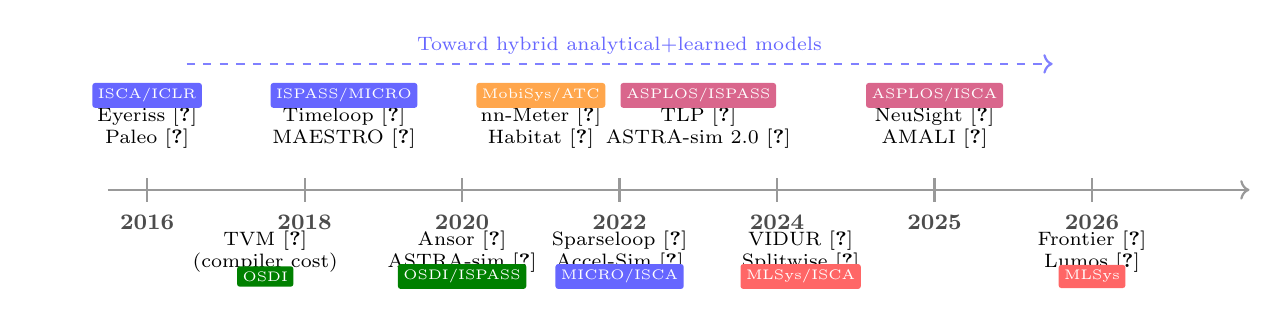
\begin{tikzpicture}[
    node distance=0.3cm,
    yearnode/.style={font=\footnotesize\bfseries, text=black!70},
    eventnode/.style={font=\scriptsize, text width=2.8cm, align=center},
    catnode/.style={font=\tiny, text=white, rounded corners=1pt, inner sep=2pt}
]
% Timeline base
\draw[thick, ->, black!40] (0,0) -- (14.5,0);

% Year markers
\foreach \x/\year in {0.5/2016, 2.5/2018, 4.5/2020, 6.5/2022, 8.5/2024, 10.5/2025, 12.5/2026} {
    \draw[thick, black!40] (\x,-0.15) -- (\x,0.15);
    \node[yearnode, below] at (\x,-0.2) {\year};
}

% Events - staggered heights to avoid overlap
% 2016: Eyeriss, Paleo
\node[eventnode, above] at (0.5,0.4) {Eyeriss~\cite{eyeriss2016}\\Paleo~\cite{paleo2017}};
\node[catnode, fill=blue!60] at (0.5,1.2) {ISCA/ICLR};

% 2018: TVM
\node[eventnode, below] at (2.0,-0.4) {TVM~\cite{tvm2018}\\(compiler cost)};
\node[catnode, fill=green!50!black] at (2.0,-1.1) {OSDI};

% 2019: Timeloop, MAESTRO
\node[eventnode, above] at (3.0,0.4) {Timeloop~\cite{timeloop2019}\\MAESTRO~\cite{maestro2019}};
\node[catnode, fill=blue!60] at (3.0,1.2) {ISPASS/MICRO};

% 2020: Ansor, ASTRA-sim
\node[eventnode, below] at (4.5,-0.4) {Ansor~\cite{ansor2020}\\ASTRA-sim~\cite{astrasim2020}};
\node[catnode, fill=green!50!black] at (4.5,-1.1) {OSDI/ISPASS};

% 2021: nn-Meter, Habitat
\node[eventnode, above] at (5.5,0.4) {nn-Meter~\cite{nnmeter2021}\\Habitat~\cite{habitat2021}};
\node[catnode, fill=orange!70] at (5.5,1.2) {MobiSys/ATC};

% 2022: Sparseloop
\node[eventnode, below] at (6.5,-0.4) {Sparseloop~\cite{sparseloop2022}\\Accel-Sim~\cite{accelsim2020}};
\node[catnode, fill=blue!60] at (6.5,-1.1) {MICRO/ISCA};

% 2023: TLP, ASTRA-sim 2.0
\node[eventnode, above] at (7.5,0.4) {TLP~\cite{tlp2023}\\ASTRA-sim 2.0~\cite{astrasim2023}};
\node[catnode, fill=purple!60] at (7.5,1.2) {ASPLOS/ISPASS};

% 2024: VIDUR, Splitwise
\node[eventnode, below] at (8.8,-0.4) {VIDUR~\cite{vidur2024}\\Splitwise~\cite{splitwise2024}};
\node[catnode, fill=red!60] at (8.8,-1.1) {MLSys/ISCA};

% 2025: NeuSight, AMALI, SimAI
\node[eventnode, above] at (10.5,0.4) {NeuSight~\cite{neusight2025}\\AMALI~\cite{amali2025}};
\node[catnode, fill=purple!60] at (10.5,1.2) {ASPLOS/ISCA};

% 2026: Frontier, Dynamic Reasoning
\node[eventnode, below] at (12.5,-0.4) {Frontier~\cite{frontier2025}\\Lumos~\cite{lumos2025}};
\node[catnode, fill=red!60] at (12.5,-1.1) {MLSys};

% Trend arrow
\draw[thick, ->, blue!50, dashed] (1,1.6) -- (12,1.6);
\node[font=\scriptsize, text=blue!60, above] at (6.5,1.6) {Toward hybrid analytical+learned models};

\end{tikzpicture}
}
\caption{Evolution of performance modeling tools for ML workloads (2016--2026). Early analytical frameworks (Eyeriss, Paleo) gave way to systematic accelerator modeling (Timeloop, MAESTRO) and distributed training simulation (ASTRA-sim). ML-augmented approaches (TVM, Habitat, NeuSight) learn performance functions from data. Recent work targets LLM-specific modeling (VIDUR, AMALI, Frontier) and large-scale training prediction (Lumos).}
\label{fig:timeline}
\end{figure}

% ==============================================================================
% SURVEY METHODOLOGY
% ==============================================================================
\section{Survey Methodology}
\label{sec:methodology}

We searched ACM Digital Library, IEEE Xplore, Semantic Scholar, and arXiv using terms related to ML performance modeling, with backward/forward citation tracking from seminal works.
Target venues include architecture (MICRO, ISCA, HPCA, ASPLOS), systems (MLSys, OSDI, SOSP, NSDI), and related (NeurIPS, MobiSys, DAC, ISPASS).
Papers must propose or evaluate a tool for predicting ML workload performance with quantitative evaluation; we exclude non-performance tasks and general-purpose workloads.
From 287 initial candidates, title/abstract screening yielded 118 papers; full-text review reduced the set to 53 that met all criteria, supplemented by 12 foundational works for context.
We cover 2016--2026 and classify each paper by \emph{methodology type} (analytical, simulation, trace-driven, ML-augmented, hybrid), \emph{target platform}, and \emph{abstraction level} (kernel, model, system).

\subsection{Related Surveys}
\label{subsec:related-surveys}

Prior surveys address adjacent topics: Rakhshanfar and Zarandi~\cite{rakhshanfar2021survey} survey ML for processor DSE; Sze et al.~\cite{sze2017efficient} treat DNN hardware design (the foundation for Timeloop/MAESTRO); GPGPU-Sim~\cite{gpgpusim2009} and gem5~\cite{binkert2011gem5} have extensive evaluation literature; and MLPerf~\cite{mlperf_training2020,mlperf_inference2020} standardizes \emph{measurement} rather than \emph{prediction}.
This survey differs by spanning the full methodology spectrum across all major platforms with hands-on reproducibility evaluations.
The closest prior work, Dudziak et al.~\cite{latencypredictorsnas2024}, compares edge device predictors for NAS; we broaden to the full landscape.

% ==============================================================================
% BACKGROUND
% ==============================================================================
\section{Background}
\label{sec:background}

\subsection{ML Workload Characteristics}
\label{subsec:workload-characteristics}

ML workloads, defined as computation graphs in frameworks like PyTorch~\cite{pytorch2019} and TensorFlow~\cite{tensorflow2016}, present distinct modeling challenges.
Their operators (convolutions, matrix multiplications, attention) have statically known shapes amenable to analytical modeling, though mixture-of-experts and dynamic inference introduce input-dependent control flow.
Performance is highly sensitive to how tensors map onto specialized memory hierarchies (dataflow, tiling, loop ordering), and for LLM inference, KV cache management dominates memory behavior~\cite{vllm2023}.
At scale, training distributes across thousands of GPUs via data, tensor, pipeline, and expert parallelism~\cite{llama3scaling2025}, requiring system-level modeling of compute--memory--network interactions.
LLM inference further splits into compute-bound prefill and memory-bound decode phases~\cite{splitwise2024}, both of which must be modeled under batched serving~\cite{sarathi2024,orca2022}.

\subsection{Modeling Methodologies}
\label{subsec:modeling-methodologies}

We classify approaches into four categories forming our taxonomy's primary axis.
\textbf{Analytical models} express performance as closed-form functions---e.g., the roofline model~\cite{williams2009roofline} bounds throughput by $P = \min(\pi, \beta \cdot I)$, while Timeloop~\cite{timeloop2019} computes data movement costs for DNN accelerator mappings. They offer microsecond evaluation but require per-architecture derivation.
\textbf{Cycle-accurate simulators} (gem5~\cite{binkert2011gem5}, GPGPU-Sim~\cite{gpgpusim2009}, Accel-Sim~\cite{accelsim2020}) achieve high fidelity but at $1000$--$10000\times$ slowdown; sampling techniques~\cite{simpoint2002,smarts2003} help but were not designed for ML workloads.
\textbf{Trace-driven simulators} like ASTRA-sim~\cite{astrasim2023} (distributed training via Chakra traces~\cite{chakra2023}) and VIDUR~\cite{vidur2024} (LLM serving) trade some fidelity for orders-of-magnitude speedup.
\textbf{ML-augmented approaches} learn performance functions from profiling data, ranging from random forests (nn-Meter~\cite{nnmeter2021}) and XGBoost (TVM~\cite{tvm2018}) to deep learning (NeuSight~\cite{neusight2025}) and meta-learning (HELP~\cite{help2021}); they capture non-linear relationships but may not generalize beyond their training distribution.

\subsection{Problem Formulation}
\label{subsec:problem-formulation}

Performance modeling maps workload $\mathcal{W}$ and hardware $\mathcal{H}$ to a metric $y$: $\hat{y} = f(\mathcal{W}, \mathcal{H}; \theta)$, with workloads represented at operator, graph, IR, or trace level, and hardware characterized by specifications, counters, or learned embeddings.
Prediction targets include latency, throughput, energy, and memory footprint.
Accuracy metrics---MAPE, RMSE, and rank correlation (Kendall's $\tau$)---vary across the literature, and differences in benchmarks, hardware targets, and evaluation protocols limit direct comparison (Section~\ref{sec:comparison}).

% ==============================================================================
% TAXONOMY
% ==============================================================================
\section{Taxonomy}
\label{sec:taxonomy}

We organize the literature along three dimensions.
The \emph{primary axis} is methodology type---how a tool predicts performance---because methodology determines the fundamental trade-offs between accuracy, speed, interpretability, and data requirements.
The \emph{secondary axes} are target platform and abstraction level, which together determine the scope and applicability of each tool.
We additionally characterize tools by workload coverage, exposing a pervasive CNN-validation bias in the literature.

Figure~\ref{fig:taxonomy-overview} illustrates the primary and secondary dimensions.
Table~\ref{tab:taxonomy-matrix} provides a unified view combining the coverage matrix (number of surveyed tools per methodology--platform cell) with trade-off profiles (evaluation speed, data requirements, interpretability, and failure modes), with empty cells highlighting research gaps.

\begin{figure}[t]
\centering
\resizebox{\columnwidth}{!}{%
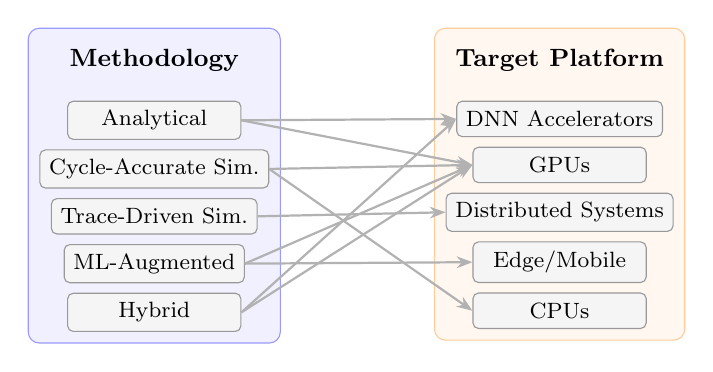
\begin{tikzpicture}[
    node distance=0.4cm and 0.6cm,
    catbox/.style={rectangle, rounded corners=2pt, draw=black!40, fill=gray!8, minimum width=2.2cm, minimum height=0.45cm, font=\footnotesize},
    dimlabel/.style={font=\small\bfseries, text=black},
    arrow/.style={-{Stealth[length=2mm]}, thick, draw=black!50}
]

% === METHODOLOGY TYPE (Left column) ===
\node[dimlabel] (meth-label) at (0, 0) {Methodology};
\node[catbox, below=0.25cm of meth-label] (analytical) {Analytical};
\node[catbox, below=0.12cm of analytical] (cycleacc) {Cycle-Accurate Sim.};
\node[catbox, below=0.12cm of cycleacc] (tracedriven) {Trace-Driven Sim.};
\node[catbox, below=0.12cm of tracedriven] (mlaugmented) {ML-Augmented};
\node[catbox, below=0.12cm of mlaugmented] (hybrid) {Hybrid};

% === TARGET PLATFORM (Right column) ===
\node[dimlabel, right=2.5cm of meth-label] (hw-label) {Target Platform};
\node[catbox, below=0.25cm of hw-label] (accel) {DNN Accelerators};
\node[catbox, below=0.12cm of accel] (gpu) {GPUs};
\node[catbox, below=0.12cm of gpu] (dist) {Distributed Systems};
\node[catbox, below=0.12cm of dist] (edge) {Edge/Mobile};
\node[catbox, below=0.12cm of edge] (cpu) {CPUs};

% === Connecting arrows showing tool-method pairings ===
% Analytical -> Accelerators (Timeloop, MAESTRO)
\draw[arrow, black!30] (analytical.east) -- (accel.west);
% Analytical -> GPU (AMALI, Roofline)
\draw[arrow, black!30] (analytical.east) -- (gpu.west);
% Cycle-accurate -> GPU (GPGPU-Sim, Accel-Sim)
\draw[arrow, black!30] (cycleacc.east) -- (gpu.west);
% Cycle-accurate -> CPU (gem5)
\draw[arrow, black!30] (cycleacc.east) -- (cpu.west);
% Trace-driven -> Distributed (ASTRA-sim, Lumos)
\draw[arrow, black!30] (tracedriven.east) -- (dist.west);
% ML-augmented -> Edge (nn-Meter, LitePred)
\draw[arrow, black!30] (mlaugmented.east) -- (edge.west);
% ML-augmented -> GPU (TVM, Ansor)
\draw[arrow, black!30] (mlaugmented.east) -- (gpu.west);
% Hybrid -> GPU (NeuSight)
\draw[arrow, black!30] (hybrid.east) -- (gpu.west);
% Hybrid -> Accelerators (ArchGym)
\draw[arrow, black!30] (hybrid.east) -- (accel.west);

% === Background boxes for each dimension ===
\begin{scope}[on background layer]
    \node[fit=(meth-label)(analytical)(cycleacc)(tracedriven)(mlaugmented)(hybrid), fill=blue!6, draw=blue!40, rounded corners=4pt, inner sep=4pt] {};
    \node[fit=(hw-label)(accel)(gpu)(dist)(edge)(cpu), fill=orange!6, draw=orange!40, rounded corners=4pt, inner sep=4pt] {};
\end{scope}

\end{tikzpicture}%
}
\caption{Primary dimensions of the taxonomy for ML workload performance modeling. The primary axis is methodology type (how performance is predicted); the secondary axis is target platform. The third dimension, abstraction level, is shown separately in Figure~\ref{fig:abstraction-levels}. Arrows show dominant pairings: analytical models for accelerators, cycle-accurate simulation for GPUs/CPUs, trace-driven simulation for distributed systems, and ML-augmented approaches for edge devices and compiler cost models.}
\label{fig:taxonomy-overview}
\end{figure}

% --- Unified Taxonomy Table (merged from Tables 1+2, issue #192) ---
\begin{table*}[t]
\centering
\caption{Methodology taxonomy: coverage matrix and trade-off profile.
Platform columns show the number of surveyed tools per cell; \textbf{0} indicates an explicit research gap.
Speed, data requirements, and interpretability determine practical applicability; the failure mode column identifies the primary condition under which each methodology breaks down.}
\label{tab:taxonomy-matrix}
\small
\begin{tabular}{l|ccccc|cccc}
\toprule
 & \textbf{DNN} & & \textbf{Distrib.} & \textbf{Edge/} & & \textbf{Eval.} & \textbf{Data} & & \textbf{Failure} \\
\textbf{Methodology} & \textbf{Accel.} & \textbf{GPU} & \textbf{Systems} & \textbf{Mobile} & \textbf{CPU} & \textbf{Speed} & \textbf{Req.} & \textbf{Interp.} & \textbf{Mode} \\
\midrule
Analytical       & 3 & 3 & 2 & \textbf{0} & \textbf{0} & $\mu$s & None & High & Dynamic effects \\
Cycle-Accurate   & 1 & 2 & \textbf{0} & \textbf{0} & 1 & Hours & Binary & High & Scale \\
Trace-Driven     & \textbf{0} & \textbf{0} & 7 & \textbf{0} & \textbf{0} & Min. & Traces & Med. & Trace fidelity \\
ML-Augmented     & \textbf{0} & 3 & \textbf{0} & 3 & 1 & ms & Profiling & Low & Distrib.\ shift \\
Hybrid           & 1 & 2 & \textbf{0} & \textbf{0} & 1 & ms & Mixed & Med. & Training domain \\
\bottomrule
\end{tabular}
\end{table*}

Table~\ref{tab:taxonomy-matrix} reveals three structural observations.
First, trace-driven simulation is exclusively used for distributed systems---no surveyed tool applies trace-driven methods to single-device GPU or accelerator modeling, despite the potential for trace-driven approaches to avoid the slowdown of cycle-accurate simulation while retaining more fidelity than analytical models.
Second, edge/mobile devices are served exclusively by ML-augmented approaches; the absence of analytical or hybrid models for edge devices reflects the hardware diversity problem but also represents a research gap, since hybrid approaches could combine the interpretability of analytical models with the adaptability of learned components.
Third, no ML-augmented or hybrid tool specifically targets distributed system modeling---tools like VIDUR use ML internally for kernel prediction but are architecturally trace-driven simulators.
The trade-off columns further show that methodologies cluster into two speed regimes: sub-millisecond (analytical, ML-augmented, hybrid) suitable for design space exploration, and minutes-to-hours (simulation, trace-driven) suitable for detailed validation.

\subsection{Primary Axis: Methodology Type}
\label{subsec:by-methodology}

The choice of methodology determines fundamental trade-offs between accuracy, evaluation speed, data requirements, and interpretability, as summarized in Table~\ref{tab:taxonomy-matrix}.

\textbf{Analytical models} express performance as closed-form functions of workload and hardware parameters.
Timeloop~\cite{timeloop2019} achieves 5--10\% error versus RTL at 2000$\times$ speedup for DNN accelerators; MAESTRO~\cite{maestro2019} and Sparseloop~\cite{sparseloop2022} extend to data-centric directives and sparse tensors; Paleo~\cite{paleo2017} and AMALI~\cite{amali2025} target distributed training and GPU LLM inference, respectively.
These models provide microsecond evaluation and full interpretability but require per-architecture derivation and may miss dynamic effects (AMALI's 23.6\% MAPE illustrates this ceiling for GPUs).

\textbf{Cycle-accurate simulators} model hardware at register-transfer level.
GPGPU-Sim~\cite{gpgpusim2009} and Accel-Sim~\cite{accelsim2020} achieve 0.90--0.97 IPC correlation; PyTorchSim~\cite{pytorchsim2025} integrates PyTorch~2 with NPU simulation.
Speed ($1000$--$10000\times$ slowdown) makes these impractical for ML design space exploration; sampling techniques~\cite{simpoint2002,smarts2003,looppoint2022} help but are unvalidated for ML workloads.

\textbf{Trace-driven simulators} replay execution traces for system-level modeling.
ASTRA-sim~\cite{astrasim2023} achieves 5--15\% error for distributed training via Chakra traces~\cite{chakra2023}; VIDUR~\cite{vidur2024} provides $<$5\% error for LLM serving; SimAI~\cite{simai2025}, Lumos~\cite{lumos2025}, and Frontier~\cite{frontier2025} target large-scale training and MoE inference.
Some tools use ML internally (e.g., VIDUR's random forests for kernel prediction), blurring the boundary with hybrid approaches.

\textbf{ML-augmented models} learn performance functions from profiling data: nn-Meter~\cite{nnmeter2021} (random forests for edge devices), LitePred~\cite{litepred2024} (85-platform transfer), HELP~\cite{help2021} (10-sample meta-learning), and TVM~\cite{tvm2018}/Ansor~\cite{ansor2020} (compiler autotuning with TenSet~\cite{tenset2021}).
Their critical failure mode is \emph{silent distribution shift}---CNN-trained models may produce confident but wrong predictions for transformers.

\textbf{Hybrid analytical+ML models} combine physics-based priors with learned residual corrections.
NeuSight~\cite{neusight2025} achieves 2.3\% MAPE on GPT-3 inference via tile-based prediction; Concorde~\cite{concorde2025} achieves 2\% CPI error on CPUs; Habitat~\cite{habitat2021} decomposes compute/memory components; ArchGym~\cite{archgym2023} connects ML surrogates to analytical simulators.
Transfer learning provides 22.5\% average improvement~\cite{latencypredictorsnas2024}.

\subsection{Secondary Axes: Platform and Abstraction Level}
\label{subsec:by-platform}

The target platform constrains applicable methodologies: \textbf{DNN accelerators}~\cite{tpuv1_2017,tpuv4_2023} are best served by analytical models (Timeloop, MAESTRO, Sparseloop) due to regular memory hierarchies; \textbf{GPUs} span the full methodology spectrum reflecting SIMT complexity; \textbf{distributed systems} require trace-driven simulation (ASTRA-sim, VIDUR, SimAI) for collective communication and pipeline parallelism; \textbf{edge/mobile devices} are dominated by ML-augmented approaches (nn-Meter, LitePred, HELP) due to hardware diversity; and \textbf{CPUs} are less studied for ML workloads (Concorde~\cite{concorde2025}, GRANITE~\cite{granite2022}).

Abstraction level determines where composition errors arise.
\textbf{Kernel-level} tools (NeuSight, nn-Meter, TVM) achieve 2--3\% error but composing predictions into end-to-end latency introduces errors from memory allocation, kernel launch overhead, and inter-operator data movement.
\textbf{Model-level} tools (Paleo, Habitat, AMALI) account for graph-level effects at 5--12\% error.
\textbf{System-level} tools (ASTRA-sim, VIDUR, SimAI) capture communication and scheduling at 5--15\% error, with kernel-level errors propagating through the composition chain.
Figure~\ref{fig:abstraction-levels} illustrates this hierarchy.

\begin{figure}[t]
\centering
\resizebox{\columnwidth}{!}{%
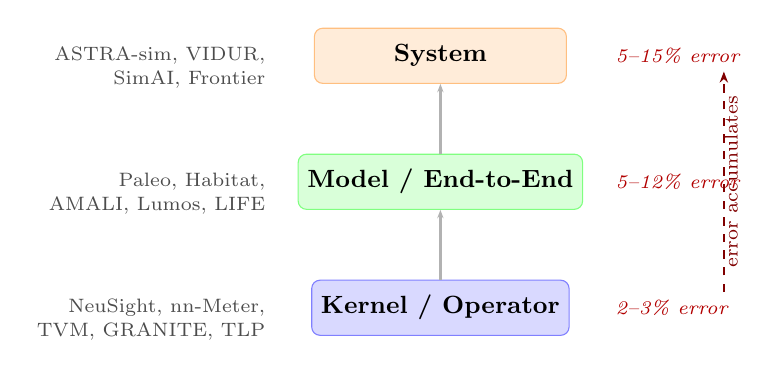
\begin{tikzpicture}[
  level/.style={draw, rounded corners=3pt, minimum width=3.2cm, minimum height=0.7cm, align=center, font=\small\bfseries},
  tool/.style={font=\scriptsize, text=black!70},
  err/.style={font=\scriptsize\itshape, text=red!70!black},
  arrow/.style={-{Stealth[length=3pt]}, thick, gray!60},
  compos/.style={-{Stealth[length=4pt]}, thick, red!50!black, dashed},
]

% Levels (bottom to top)
\node[level, fill=blue!15, draw=blue!50] (kernel) at (0,0) {Kernel / Operator};
\node[level, fill=green!15, draw=green!50] (model) at (0,1.6) {Model / End-to-End};
\node[level, fill=orange!15, draw=orange!50] (system) at (0,3.2) {System};

% Composition arrows between levels
\draw[arrow] (kernel) -- (model);
\draw[arrow] (model) -- (system);

% Tool names (left side)
\node[tool, anchor=east] at (-2.1,0) {NeuSight, nn-Meter,};
\node[tool, anchor=east] at (-2.1,-0.3) {TVM, GRANITE, TLP};
\node[tool, anchor=east] at (-2.1,1.6) {Paleo, Habitat,};
\node[tool, anchor=east] at (-2.1,1.3) {AMALI, Lumos, LIFE};
\node[tool, anchor=east] at (-2.1,3.2) {ASTRA-sim, VIDUR,};
\node[tool, anchor=east] at (-2.1,2.9) {SimAI, Frontier};

% Error ranges (right side)
\node[err, anchor=west] at (2.1,0) {2--3\% error};
\node[err, anchor=west] at (2.1,1.6) {5--12\% error};
\node[err, anchor=west] at (2.1,3.2) {5--15\% error};

% Composition problem annotation
\draw[compos] (3.6,0.2) -- (3.6,3.0);
\node[font=\scriptsize, text=red!50!black, rotate=90, anchor=south] at (3.9,1.6) {error accumulates};

\end{tikzpicture}%
}
\caption{Abstraction level hierarchy and the composition problem. Tools operate at one of three levels; composing predictions across levels accumulates error. Error ranges are representative values from surveyed papers.}
\label{fig:abstraction-levels}
\end{figure}

\subsection{Workload Coverage}
\label{subsec:workload-coverage}

Table~\ref{tab:workload-coverage} characterizes the workload types on which each tool has been validated, exposing a pervasive CNN-validation bias.

\begin{table}[t]
\centering
\caption{Workload validation coverage. \checkmark\ = validated in the original paper; $\circ$ = partial or indirect validation; --- = no validation.
Nearly all tools report accuracy on CNN workloads; transformer and MoE coverage is sparse.
Empty columns (diffusion, dynamic inference) represent workload types with \emph{no} validated performance modeling tools.}
\label{tab:workload-coverage}
\small
\begin{tabular}{lccccc}
\toprule
 & & \textbf{Trans-} & \textbf{LLM} & & \\
\textbf{Tool} & \textbf{CNN} & \textbf{former} & \textbf{Train} & \textbf{MoE} & \textbf{Diff.} \\
\midrule
Timeloop & \checkmark & $\circ$ & --- & --- & --- \\
MAESTRO & \checkmark & --- & --- & --- & --- \\
NeuSight & \checkmark & \checkmark & --- & --- & --- \\
Habitat & \checkmark & --- & --- & --- & --- \\
AMALI & --- & \checkmark & --- & --- & --- \\
ASTRA-sim & \checkmark & $\circ$ & \checkmark & --- & --- \\
VIDUR & --- & \checkmark & --- & --- & --- \\
SimAI & --- & --- & \checkmark & --- & --- \\
Lumos & --- & --- & \checkmark & --- & --- \\
Frontier & --- & \checkmark & --- & \checkmark & --- \\
nn-Meter & \checkmark & --- & --- & --- & --- \\
LitePred & \checkmark & --- & --- & --- & --- \\
HELP & \checkmark & --- & --- & --- & --- \\
TVM/Ansor & \checkmark & $\circ$ & --- & --- & --- \\
\bottomrule
\end{tabular}
\end{table}

The table reveals that \textbf{no surveyed tool has been validated on diffusion models or dynamic inference workloads}~\cite{dynamicreasoning2026}, only Frontier~\cite{frontier2025} has validated MoE support, and no single tool offers validated transformer prediction across the full kernel-to-system stack.
Practitioners working with non-CNN workloads must accept unvalidated predictions, collect their own validation data, or fall back to measurement.

% ==============================================================================
% SURVEY OF APPROACHES
% ==============================================================================
\section{Survey of Approaches}
\label{sec:survey}

This section surveys performance modeling tools for ML workloads, organized by target platform, examining modeling challenges, available tools, and their strengths and limitations.
Table~\ref{tab:survey-summary} provides a comprehensive comparison.

\begin{table*}[t]
\centering
\caption{Summary of surveyed performance modeling tools for ML workloads, organized by target platform. \textbf{Methodology}: A=Analytical, S=Simulation, T=Trace-driven, M=ML-augmented, H=Hybrid. $^*$Accuracy measures surrogate-vs-simulator fidelity, not real hardware error. $^\dagger$Reported accuracy unverifiable due to reproducibility issues. $^\ddagger$No accuracy baseline against real hardware reported.}
\label{tab:survey-summary}
\small
\begin{tabular}{lllllll}
\toprule
\textbf{Tool} & \textbf{Platform} & \textbf{Method} & \textbf{Target} & \textbf{Accuracy} & \textbf{Speed} & \textbf{Key Capability} \\
\midrule
\multicolumn{7}{l}{\textit{DNN Accelerator Modeling}} \\
Timeloop~\cite{timeloop2019} & NPU & A & Latency/Energy & 5--10\% & $\mu$s & Loop-nest DSE \\
MAESTRO~\cite{maestro2019} & NPU & A & Latency/Energy & 5--15\% & $\mu$s & Data-centric directives \\
Sparseloop~\cite{sparseloop2022} & NPU & A & Sparse tensors & 5--10\% & $\mu$s & Compression modeling \\
PyTorchSim~\cite{pytorchsim2025} & NPU & S & Cycle-accurate & N/A$^\ddagger$ & Hours & PyTorch 2 integration \\
ArchGym~\cite{archgym2023} & Multi & H & Multi-objective & 0.61\%$^*$ & ms & ML-aided DSE \\
\midrule
\multicolumn{7}{l}{\textit{GPU Performance Modeling}} \\
Accel-Sim~\cite{accelsim2020} & GPU & S & Cycle-accurate & 10--20\% & Hours & SASS trace-driven \\
GPGPU-Sim~\cite{gpgpusim2009} & GPU & S & Cycle-accurate & 10--20\% & Hours & CUDA workloads \\
AMALI~\cite{amali2025} & GPU & A & LLM inference & 23.6\% & ms & Memory hierarchy \\
NeuSight~\cite{neusight2025} & GPU & H & Kernel/E2E latency & 2.3\% & ms & Tile-based prediction \\
Habitat~\cite{habitat2021} & GPU & H & Training time & 11.8\% & Per-kernel & Wave scaling \\
\midrule
\multicolumn{7}{l}{\textit{Distributed Training and LLM Serving}} \\
ASTRA-sim~\cite{astrasim2023} & Distributed & T & Training time & 5--15\% & Minutes & Collective modeling \\
SimAI~\cite{simai2025} & Distributed & T & Training time & 1.9\% & Minutes & Full-stack simulation \\
Lumos~\cite{lumos2025} & Distributed & T & LLM training & 3.3\% & Minutes & H100 training \\
VIDUR~\cite{vidur2024} & GPU cluster & T & LLM serving & $<$5\% & Seconds & Prefill/decode phases \\
Frontier~\cite{frontier2025} & Distributed & T & MoE inference & --- & Minutes & Stage-centric sim. \\
TrioSim~\cite{triosim2025} & Multi-GPU & T & DNN training & N/A$^\ddagger$ & Minutes & Lightweight multi-GPU \\
\midrule
\multicolumn{7}{l}{\textit{Edge Device Modeling}} \\
nn-Meter~\cite{nnmeter2021} & Edge & M & Latency & $<$1\%$^\dagger$ & ms & Kernel detection \\
LitePred~\cite{litepred2024} & Edge & M & Latency & 0.7\% & ms & 85-platform transfer \\
HELP~\cite{help2021} & Multi & M & Latency & 1.9\% & ms & 10-sample adaptation \\
\midrule
\multicolumn{7}{l}{\textit{Compiler Cost Models}} \\
TVM~\cite{tvm2018} & GPU & M & Schedule perf. & $\sim$15\% & ms & Autotuning guidance \\
Ansor~\cite{ansor2020} & GPU & M & Schedule perf. & $\sim$15\% & ms & Program sampling \\
TLP~\cite{tlp2023} & GPU & M & Tensor program & $<$10\% & ms & Transformer cost model \\
\bottomrule
\end{tabular}
\end{table*}

\subsection{DNN Accelerator Modeling}
\label{subsec:accelerator-modeling}

DNN accelerators employ specialized dataflows and memory hierarchies optimized for tensor operations~\cite{sze2017efficient}, and their computational regularity makes this domain particularly amenable to analytical modeling.

\textbf{Analytical frameworks} dominate.
Timeloop~\cite{timeloop2019} computes data reuse, latency, and energy from loop-nest representations at 5--10\% error versus RTL simulation with 2000$\times$ speedup, and provides deterministic reference outputs for standard designs (Eyeriss~\cite{eyeriss2016}, Simba).
MAESTRO~\cite{maestro2019} simplifies specification via data-centric directives but is less precise for energy modeling.
Sparseloop~\cite{sparseloop2022} extends Timeloop to sparse tensors by modeling sparsity patterns, compression formats (CSR, bitmap), and hardware intersection units---critical for transformer inference but limited to static, known sparsity distributions.

\textbf{Simulation and ML-augmented approaches.}
PyTorchSim~\cite{pytorchsim2025} integrates PyTorch~2 with cycle-accurate NPU simulation, directly consuming computation graphs to eliminate manual workload translation, but does not report real-hardware accuracy and inherits simulation speed limitations.
ArchGym~\cite{archgym2023} connects ML surrogates to analytical simulators for design space exploration; its 0.61\% RMSE measures surrogate-vs-simulator fidelity, not real-hardware accuracy.
Early PIM modeling tools~\cite{upimulator2024,attacc2024,neupims2024,paise2025} target attention acceleration and PIM-GPU co-simulation but lack real PIM hardware validation (Section~\ref{sec:challenges}).

\textbf{Synthesis.}
Accelerator modeling is the most mature subdomain, with Timeloop achieving a favorable accuracy--speed--interpretability balance as the de facto DSE standard.
The progression from Timeloop through Sparseloop to PIM-aware tools illustrates a recurring pattern: each extension addresses a new workload characteristic but erodes the simplicity advantage of analytical approaches.
The key gap is silicon validation---neither ArchGym nor PyTorchSim validates against manufactured hardware, leaving all accelerator tools anchored to RTL comparisons.

\subsection{GPU Performance Modeling}
\label{subsec:gpu-modeling}

GPUs dominate ML training and inference, requiring models that account for SIMT execution, warp scheduling, memory coalescing, and occupancy effects.

\textbf{Cycle-accurate simulation.}
GPGPU-Sim~\cite{gpgpusim2009} and Accel-Sim~\cite{accelsim2020} achieve 0.90--0.97 IPC correlation; recent reverse-engineering of modern GPU cores~\cite{dissectinggpu2025} improved Accel-Sim to 13.98\% MAPE.
However, $1000$--$10000\times$ slowdown makes these tools impractical at production scale.

\textbf{Analytical models.}
The roofline model~\cite{williams2009roofline} provides upper bounds but misses dynamic effects; Roofline-LLM~\cite{rooflinellm2024} extends it to LLM inference.
AMALI~\cite{amali2025} reduces LLM inference MAPE from 127\% to 23.6\% via memory hierarchy modeling---the residual error reflects the fundamental difficulty of analytically capturing GPU dynamic behavior (warp scheduling, cache contention).

\textbf{Hybrid learned models.}
NeuSight~\cite{neusight2025} achieves 2.3\% MAPE on GPT-3 inference (H100/A100/V100) via tile-based prediction mirroring CUDA execution.
Habitat~\cite{habitat2021} uses wave scaling to decompose compute and memory components, achieving 11.8\% cross-GPU transfer error (e.g., V100$\rightarrow$A100), but requires source GPU profiling and assumes occupancy patterns remain similar across generations.
Direct comparison requires caution: NeuSight targets 2023--2025 hardware with LLMs, while Habitat was designed for earlier GPUs with CNNs.

\textbf{LLM-specific modeling.}
LLM execution exhibits distinct prefill (compute-bound) and decode (memory-bound) phases~\cite{splitwise2024,distserve2024}.
VIDUR~\cite{vidur2024} simulates LLM serving with scheduling strategies (Orca~\cite{orca2022}, Sarathi~\cite{sarathi2024}) at $<$5\% error.
LIFE~\cite{life2025} provides hardware-agnostic analytical inference modeling; HERMES~\cite{hermes2025} targets heterogeneous disaggregated serving; and emerging predictors include Omniwise~\cite{omniwise2025} and SwizzlePerf~\cite{swizzleperf2025}.

\textbf{Compiler cost models.}
TVM~\cite{tvm2018} and Ansor~\cite{ansor2020} use ML cost models for autotuning at $\sim$15\% MAPE, with TenSet~\cite{tenset2021} enabling pre-training.
TLP~\cite{tlp2023} uses transformer-based modeling for irregular workloads at $<$10\% MAPE.
SynPerf~\cite{synperf2025} uses performance models to guide kernel synthesis; both SwizzlePerf and SynPerf prioritize ranking accuracy over absolute error.

\textbf{Synthesis.}
GPU modeling exhibits the widest methodological spread: cycle-accurate simulation, analytical models, hybrid learned approaches, and LLM-based predictors all target the same hardware with error rates spanning 2\%--24\%.
This diversity reflects the fundamental tension between microarchitectural complexity (making analytical modeling hard) and rapid hardware evolution (invalidating training data for learned approaches).
NeuSight currently offers the best accuracy--speed trade-off for LLM workloads, but per-GPU profiling limits pre-silicon use---a gap that AMALI and LIFE fill despite higher error.
The compiler cost model ecosystem (TVM, TLP, SynPerf) represents a distinct use case where relative ranking matters more than absolute prediction.

\subsection{Distributed Training and LLM Serving}
\label{subsec:distributed-modeling}

Distributed systems introduce communication overhead, synchronization barriers, and parallelism strategy choices across tensor~\cite{megatronlm2020}, pipeline~\cite{gpipe2019}, and data parallelism with memory-efficient optimizers~\cite{zero2020}.

\textbf{Training simulation.}
ASTRA-sim~\cite{astrasim2023} provides end-to-end training simulation via Chakra traces~\cite{chakra2023} at 5--15\% error versus HGX-H100 clusters.
SimAI~\cite{simai2025} achieves 1.9\% MAPE at Alibaba Cloud scale; Lumos~\cite{lumos2025} achieves 3.3\% error on H100 training; Echo~\cite{echo2024} and TrioSim~\cite{triosim2025} offer additional training simulation approaches.
PRISM~\cite{prism2025} produces prediction intervals at 10K+ GPU scale, capturing stochastic variation.

\textbf{Scaling and parallelism.}
Paleo~\cite{paleo2017} pioneered analytical training-time estimation; MAD Max~\cite{madmax2024} extends this per parallelism dimension.
The Llama~3 scaling study~\cite{llama3scaling2025} documents 4D parallelism at 16K H100 GPUs as validation ground truth.
Sailor~\cite{sailor2025} addresses parallelism selection over heterogeneous clusters.

\textbf{Inference serving.}
VIDUR~\cite{vidur2024} extends to distributed serving with vLLM~\cite{vllm2023} scheduling; Frontier~\cite{frontier2025} targets MoE and disaggregated inference; ThrottLL'eM~\cite{throttllem2025} models GPU power management effects on inference.
KV cache management is the key serving bottleneck (vLLM's PagedAttention~\cite{vllm2023} achieves 2--4$\times$ throughput), modeled by VIDUR at the system level; low-level memory simulators (DRAMSim3~\cite{dramsim3_2020}, Ramulator~2~\cite{ramulator2_2023}) integrate with tools like Accel-Sim for detailed memory modeling.
Algorithmic innovations like speculative decoding~\cite{medusa2024} create a moving-target challenge for all serving simulators.

\textbf{Synthesis.}
Distributed modeling is the fastest-growing subdomain, bifurcating into \emph{trace-driven fidelity} (ASTRA-sim, SimAI) and \emph{analytical decomposition} (Paleo, MAD Max), with PRISM's probabilistic approach as an emerging third path.

\subsection{Edge Device Modeling}
\label{subsec:edge-modeling}

Edge devices impose strict power, memory, and latency constraints, and their hardware diversity (mobile CPUs, GPUs, NPUs, DSPs) makes per-device analytical modeling impractical, driving ML-augmented approaches.

nn-Meter~\cite{nnmeter2021} reports $<$1\% MAPE using random forest ensembles, but this claim is unverifiable: pre-trained predictors fail with modern scikit-learn versions, scoring 3/10 in our reproducibility evaluation.
LitePred~\cite{litepred2024} achieves 0.7\% MAPE across 85 platforms using VAE-based intelligent sampling that reduces adaptation to under one hour per device, though the platforms are predominantly ARM-based and transfer to NPUs/DSPs likely degrades.
HELP~\cite{help2021} achieves 1.9\% MAPE with MAML-style 10-sample adaptation, though accuracy depends on selecting representative operators for the target workload.
ESM~\cite{esm2025} systematically evaluates surrogate models for hardware-aware NAS, finding that well-tuned random forests match deep learning surrogates---suggesting the field may over-invest in model complexity relative to data quality.
The latency predictor study~\cite{latencypredictorsnas2024} shows transfer learning provides 22.5\% average improvement, up to 87.6\% on challenging cross-platform transfers.

\textbf{Synthesis.}
Edge modeling is dominated by ML-augmented approaches, with the central challenge being \emph{generalization} to new devices with minimal profiling.
ESM's finding that simple models match complex ones, combined with nn-Meter's reproducibility failure, suggests that data quality and tool longevity matter more than model sophistication.

\subsection{Cross-Cutting Themes}
\label{subsec:cross-cutting}

Several themes cut across platform categories.
\emph{Structural decomposition} mirroring hardware execution outperforms black-box approaches (Timeloop's loop nests, NeuSight's tiles, VIDUR's prefill/decode separation), while modular pluggable backends (ASTRA-sim, VIDUR) enable adoption.
\emph{Verifiable moderate accuracy} matters more than \emph{unverifiable high accuracy}---Timeloop (9/10 reproducibility) and ASTRA-sim (8.5/10) see sustained adoption, while nn-Meter ($<$1\% MAPE claimed, 3/10 reproducibility) sees decline.

A persistent \textbf{accuracy--generality--speed trilemma} explains why no single methodology has displaced others: cycle-accurate simulators maximize accuracy but sacrifice speed; analytical models maximize speed but sacrifice accuracy on complex hardware; ML-augmented approaches achieve both but sacrifice generality, requiring retraining when hardware changes.
The maturity of each subdomain mirrors economic incentive: accelerator DSE is most mature (irreversible chip design errors), distributed training simulation is fastest-growing (million-dollar training runs), and edge modeling has weakest reproducibility (lower deployment costs).

% ==============================================================================
% COMPARISON AND ANALYSIS
% ==============================================================================
\section{Comparison and Analysis}
\label{sec:comparison}

We analyze trade-offs across methodology types along accuracy and speed dimensions (see Table~\ref{tab:survey-summary} for per-tool details); generalization and interpretability challenges are deferred to Section~\ref{sec:challenges}.

\subsection{Accuracy by Problem Difficulty}
\label{subsec:accuracy-difficulty}

We organize accuracy results by inherent problem difficulty rather than comparing across incompatible benchmarks (Figure~\ref{fig:accuracy-comparison}).
Accelerator dataflow modeling is most tractable (Timeloop: 5--10\%); single-GPU kernel prediction achieves 2--12\% via hybrid methods (NeuSight, Habitat); distributed systems reach 2--15\% (SimAI 1.9\%, ASTRA-sim 5--15\%); cross-platform edge prediction achieves 0.7--2\% but requires per-device profiling; and GPU analytical modeling remains hardest (AMALI: 23.6\%).
Setup costs vary dramatically: analytical models require only architecture specifications, ML-augmented approaches need 10--10K profiling samples per device, and cycle-accurate simulators require hardware-specific binaries or traces.

\begin{figure}[t]
\centering
\resizebox{\columnwidth}{!}{%
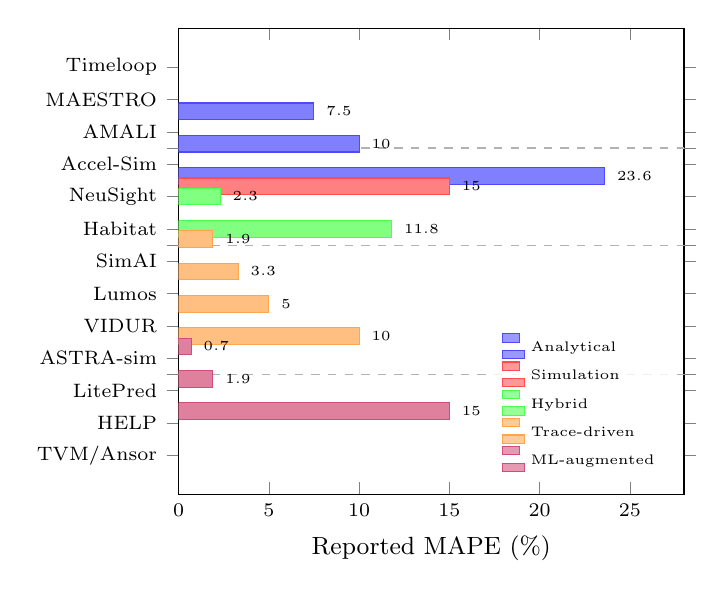
\begin{tikzpicture}
\begin{axis}[
    xbar,
    y dir=reverse,
    xlabel={Reported MAPE (\%)},
    xmin=0, xmax=28,
    ytick={0,1,2,3,4,5,6,7,8,9,10,11,12},
    yticklabels={
        Timeloop,
        MAESTRO,
        AMALI,
        Accel-Sim,
        NeuSight,
        Habitat,
        SimAI,
        Lumos,
        VIDUR,
        ASTRA-sim,
        LitePred,
        HELP,
        TVM/Ansor
    },
    yticklabel style={font=\scriptsize},
    xticklabel style={font=\scriptsize},
    xlabel style={font=\small},
    bar width=6pt,
    height=7.5cm,
    width=8cm,
    nodes near coords,
    nodes near coords style={font=\tiny, anchor=west},
    every node near coord/.append style={xshift=1pt},
    legend style={at={(0.97,0.03)}, anchor=south east, font=\tiny, draw=none, fill=white, fill opacity=0.8, text opacity=1},
    legend cell align={left},
    extra y ticks={2.5, 5.5, 9.5},
    extra y tick labels={},
    extra y tick style={grid=major, grid style={black!30, dashed}},
]
% Analytical (blue)
\addplot[fill=blue!50, draw=blue!70] coordinates {(7.5,0) (10,1) (23.6,2)};
% Simulation (red)
\addplot[fill=red!50, draw=red!70] coordinates {(15,3)};
% Hybrid (green)
\addplot[fill=green!50, draw=green!70] coordinates {(2.3,4) (11.8,5)};
% Trace-driven (orange)
\addplot[fill=orange!50, draw=orange!70] coordinates {(1.9,6) (3.3,7) (5,8) (10,9)};
% ML-augmented (purple)
\addplot[fill=purple!50, draw=purple!70] coordinates {(0.7,10) (1.9,11) (15,12)};
\legend{Analytical, Simulation, Hybrid, Trace-driven, ML-augmented}
\end{axis}
\end{tikzpicture}%
}
\caption{Reported accuracy (MAPE) of surveyed tools, grouped by methodology type. Range midpoints used where ranges are reported. Cross-tool comparison is approximate due to differing benchmarks, workloads, and hardware targets.}
\label{fig:accuracy-comparison}
\end{figure}

\subsection{Practitioner Tool Selection}
\label{subsec:tool-selection}

Figure~\ref{fig:decision-flowchart} presents a decision flowchart for tool selection based on platform and use case.

\begin{figure}[t]
\centering
\resizebox{\columnwidth}{!}{%
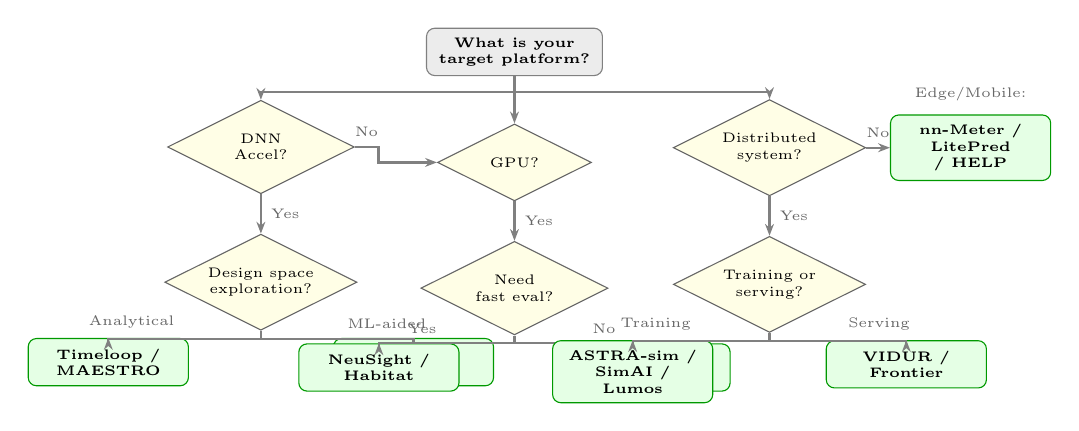
\begin{tikzpicture}[
    node distance=0.5cm and 0.3cm,
    decision/.style={diamond, draw=black!60, fill=yellow!10, text width=1.5cm, align=center, inner sep=1pt, font=\tiny, aspect=2},
    block/.style={rectangle, rounded corners=3pt, draw=black!50, fill=blue!8, text width=2.0cm, align=center, minimum height=0.6cm, font=\tiny},
    result/.style={rectangle, rounded corners=3pt, draw=green!60!black, fill=green!10, text width=1.8cm, align=center, minimum height=0.6cm, font=\tiny\bfseries},
    arr/.style={-{Stealth[length=1.5mm]}, thick, draw=black!50},
    lbl/.style={font=\tiny, text=black!60}
]
\node[block, fill=gray!15, font=\tiny\bfseries] (start) {What is your target platform?};
\node[decision, below left=0.6cm and 1.5cm of start] (accel) {DNN\\Accel?};
\node[decision, below=0.6cm of start] (gpu) {GPU?};
\node[decision, below right=0.6cm and 1.5cm of start] (dist) {Distributed\\system?};
\draw[arr] (start.south) -- ++(0,-0.2) -| (accel.north);
\draw[arr] (start.south) -- (gpu.north);
\draw[arr] (start.south) -- ++(0,-0.2) -| (dist.north);
\node[decision, below=0.5cm of accel] (accel-dse) {Design space\\exploration?};
\draw[arr] (accel.south) -- node[lbl,right]{Yes} (accel-dse.north);
\node[result, below left=0.4cm and 0.3cm of accel-dse] (r-timeloop) {Timeloop /\\MAESTRO};
\node[result, below right=0.4cm and 0.3cm of accel-dse] (r-archgym) {ArchGym};
\draw[arr] (accel-dse.south) -- ++(0,-0.1) -| node[lbl,above left,pos=0.25]{Analytical} (r-timeloop.north);
\draw[arr] (accel-dse.south) -- ++(0,-0.1) -| node[lbl,above right,pos=0.25]{ML-aided} (r-archgym.north);
\node[decision, below=0.5cm of gpu] (gpu-speed) {Need\\fast eval?};
\draw[arr] (gpu.south) -- node[lbl,right]{Yes} (gpu-speed.north);
\node[result, below left=0.4cm and 0.1cm of gpu-speed] (r-neusight) {NeuSight /\\Habitat};
\node[result, below right=0.4cm and 0.1cm of gpu-speed] (r-accelsim) {Accel-Sim /\\GPGPU-Sim};
\draw[arr] (gpu-speed.south) -- ++(0,-0.1) -| node[lbl,above left,pos=0.25]{Yes} (r-neusight.north);
\draw[arr] (gpu-speed.south) -- ++(0,-0.1) -| node[lbl,above right,pos=0.25]{No} (r-accelsim.north);
\node[decision, below=0.5cm of dist] (dist-type) {Training or\\serving?};
\draw[arr] (dist.south) -- node[lbl,right]{Yes} (dist-type.north);
\node[result, below left=0.4cm and 0.1cm of dist-type] (r-astra) {ASTRA-sim /\\SimAI / Lumos};
\node[result, below right=0.4cm and 0.1cm of dist-type] (r-vidur) {VIDUR /\\Frontier};
\draw[arr] (dist-type.south) -- ++(0,-0.1) -| node[lbl,above left,pos=0.25]{Training} (r-astra.north);
\draw[arr] (dist-type.south) -- ++(0,-0.1) -| node[lbl,above right,pos=0.25]{Serving} (r-vidur.north);
\node[result, right=0.3cm of dist] (r-edge) {nn-Meter /\\LitePred / HELP};
\node[lbl, above=0.05cm of r-edge] {Edge/Mobile:};
\draw[arr] (accel.east) -- node[lbl,above]{No} ++(0.3,0) |- (gpu.west);
\draw[arr] (dist.east) -- node[lbl,above]{No} (r-edge.west);
\end{tikzpicture}%
}
\caption{Practitioner decision flowchart for tool selection. Platform determines the candidate set; speed and use case narrow the choice.}
\label{fig:decision-flowchart}
\end{figure}

Three recommendations:
(1)~For \emph{accelerator DSE}, use Timeloop or MAESTRO for microsecond-speed exhaustive search with interpretable bottleneck feedback.
(2)~For \emph{GPU evaluation}, NeuSight offers the best accuracy--speed balance for LLMs; use Accel-Sim when microarchitectural detail is needed.
(3)~For \emph{distributed systems}, use VIDUR for LLM serving configuration and ASTRA-sim or SimAI for training parallelism at scale.

% ==============================================================================
% EXPERIMENTAL EVALUATION
% ==============================================================================
\section{Experimental Evaluation}
\label{sec:evaluation}

We conducted hands-on evaluations of five tools spanning methodology types: Timeloop (analytical), ASTRA-sim (trace-driven, distributed), VIDUR (trace-driven, LLM serving), nn-Meter (ML-augmented, edge), and NeuSight (hybrid, GPU).

\textbf{Environment and rubric.}
All evaluations ran on Apple M2 Ultra (aarch64, 192\,GB RAM) using Docker containers where provided---no GPU hardware was available, so we cannot validate absolute accuracy claims.
We score each tool on a 10-point rubric: \emph{Setup} (3 pts), \emph{Reproducibility} (4 pts), \emph{Usability} (3 pts).
Table~\ref{tab:evaluation-summary} summarizes results.

\begin{table}[t]
\centering
\caption{Reproducibility evaluation scores (10-point rubric). Tools are ranked by total score. $^\dagger$Timeloop CLI works but Python bindings fail.}
\label{tab:evaluation-summary}
\small
\begin{tabular}{lcccc}
\toprule
\textbf{Tool} & \textbf{Setup} & \textbf{Reprod.} & \textbf{Usability} & \textbf{Total} \\
\midrule
VIDUR & 2.5 & 3.5 & 3 & 9/10 \\
Timeloop$^\dagger$ & 3 & 4 & 2 & 9/10 \\
ASTRA-sim & 2.5 & 3 & 3 & 8.5/10 \\
NeuSight & 2 & 3 & 2.5 & 7.5/10 \\
nn-Meter & 2 & 0 & 1 & 3/10 \\
\bottomrule
\end{tabular}
\end{table}

\subsection{Per-Tool Results}
\label{subsec:per-tool-results}

\textbf{VIDUR} (9/10)---the highest-scoring tool.
We simulated Llama-2-7B inference on a simulated A100 using vLLM and Sarathi scheduling (Table~\ref{tab:vidur-results}).
VIDUR correctly captures scheduling trade-offs: Sarathi achieves 12.2\% lower latency than vLLM (0.158\,s vs.\ 0.177\,s) via chunked prefill~\cite{sarathi2024}, TPOT differs by only 3.5\% (confirming hardware-bound decode), and vLLM preempted 26.5\% of requests while Sarathi preempted zero---matching the algorithmic difference in KV-cache management~\cite{vllm2023}.
VIDUR's Docker-pinned dependencies avoid the serialization failures seen in nn-Meter.

\begin{table}[t]
\centering
\caption{VIDUR simulation results for Llama-2-7B inference serving on a simulated A100 GPU. All metrics from our own experiments.}
\label{tab:vidur-results}
\small
\begin{tabular}{lcc}
\toprule
\textbf{Metric} & \textbf{vLLM} & \textbf{Sarathi} \\
\midrule
Requests & 200 & 50 \\
Avg E2E latency (s) & 0.177 & 0.158 \\
P99 E2E latency (s) & 0.320 & 0.270 \\
Avg TTFT (s) & 0.027 & 0.025 \\
Avg TPOT (s) & 0.0093 & 0.0090 \\
Requests preempted & 53 & 0 \\
\bottomrule
\end{tabular}
\end{table}

\textbf{Timeloop} (9/10).
The Docker image provides CLI tools that work correctly for Eyeriss-like configurations with fully deterministic, bit-identical outputs---a significant reproducibility strength.
Reference outputs for standard designs (Eyeriss, Simba) enable verification without hardware.
However, Python bindings fail (\texttt{ImportError: libbarvinok.so.23}), preventing programmatic use.

\textbf{ASTRA-sim} (8.5/10).
We executed 8-NPU collective microbenchmarks and ResNet-50 data-parallel training at 2--8 GPUs on HGX-H100 (Table~\ref{tab:astrasim-results}).
Collective operation ratios are physically plausible: Reduce-Scatter takes half the time of All-Reduce (consistent with half the data), while All-to-All takes $\sim$2$\times$ All-Reduce.
Communication overhead scales from 0.05\% (2 GPUs) to 0.30\% (8 GPUs)---a 5.76$\times$ increase for 4$\times$ more GPUs, consistent with ring All-Reduce scaling.
Scale coverage is limited to 8 NPUs by included topology files.

\begin{table}[t]
\centering
\caption{ASTRA-sim quantitative results from our experiments on the HGX-H100 configuration. Top: collective microbenchmarks (8 NPUs, 1\,MB). Bottom: ResNet-50 data-parallel training scaling.}
\label{tab:astrasim-results}
\small
\begin{tabular}{lrr}
\toprule
\multicolumn{3}{l}{\textbf{Collective Microbenchmarks (8 NPUs, 1\,MB)}} \\
\midrule
\textbf{Collective} & \textbf{Cycles} & \textbf{Ratio vs.\ AR} \\
\midrule
All-Reduce & 57,426 & 1.000 \\
All-Gather & 44,058 & 0.767 \\
Reduce-Scatter & 28,950 & 0.504 \\
All-to-All & 114,000 & 1.985 \\
\midrule
\multicolumn{3}{l}{\textbf{ResNet-50 Data-Parallel Training}} \\
\midrule
\textbf{GPUs} & \textbf{Comm Cycles} & \textbf{Comm Overhead} \\
\midrule
2 & 574,289 & 0.05\% \\
4 & 1,454,270 & 0.13\% \\
8 & 3,307,886 & 0.30\% \\
\bottomrule
\end{tabular}
\end{table}

\textbf{NeuSight} (7.5/10).
The tile-based decomposition correctly mirrors CUDA tiling for standard dense operations, but testing on irregular workloads was limited by missing examples, suggesting the tool is best validated for regular LLM workloads.

\textbf{nn-Meter} (3/10)---the lowest-scoring tool.
After four installation attempts ($>$4 hours), we could not execute \emph{any} predictions due to a chain of unpinned dependencies: pickle-serialized predictors (scikit-learn 0.23.1) are incompatible with current versions, and onnx-simplifier fails on aarch64.
The claimed $<$1\% MAPE is \textbf{unverifiable on any current software stack}; the tool has received no updates since 2022.

\subsection{Lessons and Threats to Validity}
\label{subsec:eval-lessons}

Five lessons emerge:
(1)~\textbf{Docker-first deployment} is the strongest reproducibility predictor (Docker tools: 8.5+/10; nn-Meter without Docker: 3/10).
(2)~\textbf{ML model serialization is fragile}---nn-Meter's pickle-based predictors became unusable within two years.
(3)~\textbf{Reference outputs enable trust without hardware}---Timeloop and ASTRA-sim include verifiable baselines.
(4)~\textbf{Scale-limited evaluation understates system tools}---our 2--8 GPU tests show only 0.30\% communication overhead, far below production scales~\cite{llama3scaling2025}.
(5)~\textbf{Reproducible accuracy claims should be weighted higher} than unreproducible ones.

\textbf{Threats.}
Our venue-focused search may under-represent industry and non-English publications; we exclude proprietary tools (Nsight Compute, internal TPU models); and accuracy metrics vary across papers (MAPE, RMSE, Kendall's $\tau$), limiting direct comparison.

% ==============================================================================
% OPEN CHALLENGES
% ==============================================================================
\section{Open Challenges and Future Directions}
\label{sec:challenges}

\textbf{Generalization gaps.}
Three dimensions of generalization remain largely unsolved.
\emph{Workload generalization}: nearly all accuracy numbers are measured on CNNs, with CNN$\rightarrow$transformer transfer largely unvalidated (NeuSight is a notable exception); MoE, diffusion models, and dynamic inference~\cite{dynamicreasoning2026} have almost no validated prediction tools.
Neural scaling laws~\cite{kaplan2020scaling,hoffmann2022chinchilla,scalinglaws2024,scalinglawguide2025} predict training loss but not hardware-specific latency.
Figure~\ref{fig:workload-coverage} shows the shift from CNN-only validation toward LLM workloads since 2023, but MoE and diffusion remain uncharacterized.
\emph{Hardware generalization}: meta-learning (HELP: 10-sample adaptation), feature-based transfer (LitePred: 85 devices), and analytical decomposition (Habitat) show promise, but cross-family transfer (GPU$\rightarrow$TPU$\rightarrow$PIM) remains unsolved.
\emph{Temporal generalization}---software stack evolution silently invalidating trained models---is addressed by no surveyed tool.

\begin{figure}[t]
\centering
\resizebox{\columnwidth}{!}{%
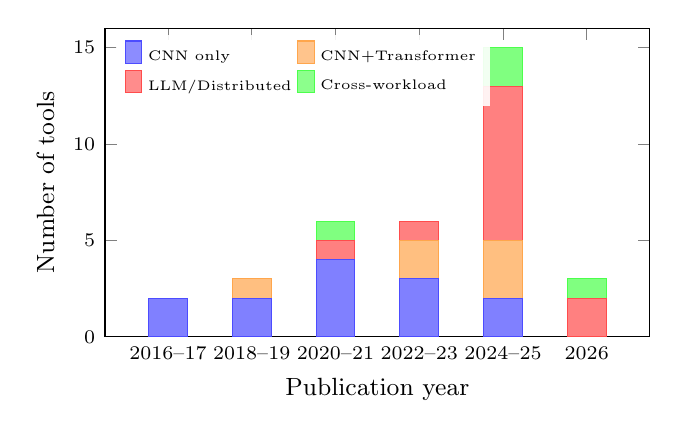
\begin{tikzpicture}
\begin{axis}[
    ybar stacked,
    bar width=14pt,
    xlabel={Publication year},
    ylabel={Number of tools},
    ymin=0, ymax=16,
    xtick={2016,2018,2020,2022,2024,2026},
    xticklabels={2016--17,2018--19,2020--21,2022--23,2024--25,2026},
    xticklabel style={font=\scriptsize},
    yticklabel style={font=\scriptsize},
    xlabel style={font=\small},
    ylabel style={font=\small},
    legend style={at={(0.02,0.98)}, anchor=north west, font=\tiny, draw=none, fill=white, fill opacity=0.9, text opacity=1, legend columns=2},
    legend cell align={left},
    height=5.5cm,
    width=8.5cm,
    enlarge x limits={abs=0.8cm},
]
\addplot[fill=blue!50, draw=blue!70] coordinates {(2016,2) (2018,2) (2020,4) (2022,3) (2024,2) (2026,0)};
\addplot[fill=orange!50, draw=orange!70] coordinates {(2016,0) (2018,1) (2020,0) (2022,2) (2024,3) (2026,0)};
\addplot[fill=red!50, draw=red!70] coordinates {(2016,0) (2018,0) (2020,1) (2022,1) (2024,8) (2026,2)};
\addplot[fill=green!50, draw=green!70] coordinates {(2016,0) (2018,0) (2020,1) (2022,0) (2024,2) (2026,1)};
\legend{CNN only, CNN+Transformer, LLM/Distributed, Cross-workload}
\end{axis}
\end{tikzpicture}%
}
\caption{Workload coverage of surveyed tools by publication period. The shift toward transformer and LLM workloads accelerates from 2023, but MoE and diffusion models remain largely uncharacterized.}
\label{fig:workload-coverage}
\end{figure}

\textbf{The composition problem.}
Composing kernel-level predictions into end-to-end estimates is unsolved: NeuSight's 2.3\% kernel MAPE yields $\sim$$10\times$ higher variance at model level ($\sigma_{\text{model}} \approx \sigma_{\text{kernel}} \cdot \sqrt{N}$), and correlated errors can compound linearly.
VIDUR sidesteps this by profiling entire prefill/decode phases.

\textbf{Emerging hardware and reproducibility.}
PIM architectures~\cite{upimulator2024,attacc2024,neupims2024,paise2025}, chiplets, and disaggregated designs blur conventional memory hierarchy assumptions; hardware-aware optimizations (FlashAttention~\cite{flashattention2022}) change the performance landscape faster than models can be retrained.
On the reproducibility front, no equivalent of MLPerf~\cite{mlperf_training2020,mlperf_inference2020} exists for performance \emph{prediction}---standardized prediction benchmarks would significantly advance the field.
Analytical models remain the most interpretable: Timeloop identifies data movement bottlenecks, MAESTRO reveals suboptimal dataflows, and VIDUR exposes scheduling inefficiencies, while ML-augmented approaches offer limited causal understanding.

\textbf{Future directions.}
Five priorities: (1)~transformer/MoE-aware tools with validated non-CNN accuracy; (2)~validated composition methods with bounded end-to-end error; (3)~unified energy-latency-memory prediction~\cite{mlperfpower2025}; (4)~temporal robustness benchmarks for software stack evolution; (5)~unified tooling with Docker-first deployment, portable formats (ONNX), and standard workload representations (Chakra~\cite{chakra2023}).

% ==============================================================================
% CONCLUSION
% ==============================================================================
\section{Conclusion}
\label{sec:conclusion}

This survey analyzed over 30 tools for predicting ML workload performance, organized by methodology type, target platform, and abstraction level.
Key findings:
(1)~\emph{Methodology determines trade-offs, not quality}---analytical models offer microsecond interpretable evaluation, trace-driven simulators provide 2--15\% system-level error, and hybrid approaches achieve the best accuracy--speed balance (NeuSight: 2.3\% MAPE).
(2)~\emph{LLM workloads demand specialized modeling}---prefill/decode distinctions, KV cache management, and dynamic batching require purpose-built tools (VIDUR, Frontier) rather than CNN-era extensions.
(3)~\emph{Reproducibility is a practical bottleneck}---Docker-first tools score 8.5+/10 while tools relying on serialized ML models have become unusable.
(4)~\emph{Accuracy claims require scrutiny} due to varying benchmarks and metrics.

The most pressing gaps are CNN-to-transformer generalization, kernel-to-end-to-end composition, emerging hardware support (PIM, chiplets), and reproducibility failures.
As ML workloads grow in scale and diversity, this survey provides practitioners guidance for tool selection and researchers a roadmap for advancing the field.

%%%%%%% -- PAPER CONTENT ENDS -- %%%%%%%%

%%
%% The next two lines define the bibliography style to be used, and
%% the bibliography file.
\bibliographystyle{ACM-Reference-Format}
\bibliography{references}

\end{document}
